% !Mode:: "TeX:UTF-8"
\chapter{开发环境}

\begin{introduction}
	\item 开发环境
	\item 安装JDK
	\item 安装IDE
\end{introduction}

本书使用Java语言介绍机器学算法,所有的演示代码可在JDK8以上正常运行。
在开始学习之前,请先安装JDK(Java Development Kit)和IDE(Integrated Development Environment)。

\begin{table}[!htbp]\centering
	\caption{开发环境}
	\begin{tabular}{|p{1cm}|p{3cm}|p{8cm}|}
	\toprule
	序号 & \multicolumn{2}{|c|}{开发环境}\\
	\midrule
	1. & JDK8+&建议Oracle JDK\\
	\hline
	2. & IntelliJ IDEA&界面友好,操作简单\\
	\hline
	3. & VSCode&强大开源,插件众多\\
	\hline
	4. & ND4J&Java实现的矩阵/向量支持库\\
	\hline
	5. & DL4J&开源机器学习Java实现\\
	\bottomrule
	\end{tabular}
	\label{tab:part1_dev_env}
\end{table}

\section{安装JDK}
安装JDK(Java Development Kit),有2个选择:Oracle JDK和Open JDK。
在本书中,你可以无视它们两者之间的差异。
使用Linux系统的同学,保持Open JDK即可。
值得注意的是,近年来关于Oracle JDK的纠纷越来越多,
实际上,在Sun被Oracle收购之前,JDK也是要授权费的,但很少有公司愿意支付这笔费用。

\begin{table}[!htbp]\centering \small
	\begin{tabular}{cc|c|ccc|c|cc}
		\toprule
		输入&&编译&&输出&&执行&&输出 \\
		\midrule
		Hello.java&=>&javac&=>&Hello.class&=>&java&=>&输出 \\
		&&JDK&&&&JRE&& \\
		\bottomrule
	\end{tabular}
\end{table}

JRE(Java Runtime Environment)是Java程序的运行环境,不要下载错了。
安装JDK的过程中,全部默认点选“下一步”即可。
结束后,需要手动配置以下2个环境变量:JAVA\_HOME、CLASSPATH。
配置环境变量的主要目的是告诉IDE或系统,在哪里能找到某个程序或文件。
把JAVA\_HOME
设定为JDK的安装目录,进一步在此基础上添加bin目录到环境变量。
如果没有配置,或者设置不正确,在控制台(cmd、bash)就会提示错误。
\begin{lstlisting}[language=bash]
	# Ubuntu
	parallels@ubuntu-vm:~$ java
	Command 'java' not found, but can be installed with:

	# Windows
	C:\Users\simbaba>java
	'java' 不是内部或外部命令,也不是可运行的程序
	或批处理文件。
\end{lstlisting}

Windows上的配置相对比较简单,参考下图打开环境变量配置窗口。
选择系统环境变量或者帐号环境变量里面都可以,区别是系统环境变量会影响所有用户。
通常建议修改帐号环境变量,有些帐号可能也没权限修改系统环境变量。
在其中,新建2个条目:
\begin{enumerate}
	\item JAVA\_HOME, java的安装目录
	\item 在path后面追加, \text{\%JAVA\_HOME\%}$\backslash$bin
\end{enumerate}

\begin{figure}[!htb]
	\centerline{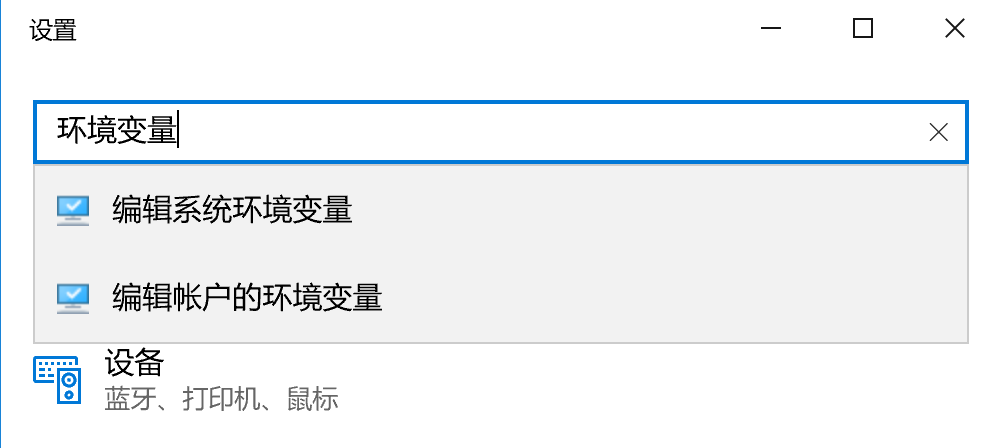
\includegraphics[width=.4\figwidth]{images/windows_java_home.png}}
\end{figure}

Linux和Mac的配资方法大致相同,需要修改配置文件。
\footnote{.bash\_profile、.bashrc或.profile等。}
\begin{lstlisting}[language=bash]
	# Mac、Linux
	export JAVA_HOME= JAVA安装目录
	export path=$PATH:$JAVA_HOME/bin
\end{lstlisting}

\section{安装IDE}
目前主流的IDE有:Eclipse、IDEA、VSCode。